\documentclass{beamer}

% If you use the optional handout parameter below, none of the pauses between slides are printed.  Only one of these first two lines should be used at a time.
%\documentclass[handout]{beamer}

\usepackage{amsmath, amsthm, amssymb, upgreek,amscd, verbatim, xcolor}
\usepackage{centernot}
\usepackage{datetime}

\usetheme{Warsaw}
\setbeamertemplate{items}[circle]
\setbeamertemplate{navigation symbols}{}
\usefonttheme{serif}
\usepackage{tabmac}
\usepackage{graphicx}


%New Commands
\newcommand{\ssm}{\,{}^\smallsetminus\,}
\newcommand{\R}{\mathbb{R}}
\newcommand{\Q}{\mathbb{Q}}
\newcommand{\Z}{\mathbb{Z}}
\newcommand{\N}{\mathbb{N}}
\newcommand{\F}{\mathbb{F}}



%Date
%\newdateformat{mydate}{\THEDAY \ \monthname[\THEMONTH] \THEYEAR}

\begin{document}
\title[Equivariant Rim Hook Rule]{A rim hook rule for the equivariant quantum cohomology of the Grassmannian}
\author[Elizabeth Mili\'cevi\'c]{\textcolor{blue}{Elizabeth Mili\'cevi\'c\\ Haverford College}}
%\institute{Haverford College}
%\date{\mydate\today}
%\date{}

\date{joint work with\\ Anna Bertiger (University of Waterloo) and \\ Kaisa Taipale (University of Minnesota)}



\begin{frame}
\titlepage

\begin{center}
\textcolor{blue}{arXiv.org/1403.6218}
\end{center}
\end{frame}




%-------------------------------------------%


\begin{frame}{Cohomology: A First Example}

Consider projective space $\mathbb{P}^3$.  Intersection theory is encoded by the cup product in \emph{cohomology}.  \pause The cohomology of $\mathbb{P}^3$ has
a basis indexed by the following \emph{Young diagrams}:
\[ \mathrm{whole \;space} \; = \emptyset, \;\; \mathrm{plane} \; = \tableau[Ys]{ \\}, \;\; \mathrm{line} \; = \tableau[Ys]{ & \\}, \;  \;\mathrm{point} \;= \tableau[Ys]{ & & \\} \]

\pause
These representations allow us to compute products as ``box addition''.
Intuitively, think about intersections in 3D space.

\medskip

\begin{displaymath}\tableau[Ys]{ \\} \cdot \tableau[Ys]{ \\} =
  \tableau[Ys]{ & \\}\end{displaymath}
\pause
\[\tableau[Ys]{ \\} \cdot \tableau[Ys]{ & \\} = \tableau[Ys]{ & &
  \\}\]
\pause
\[\tableau[Ys]{ \\} \cdot \tableau[Ys]{ & & \\} = 0 \]



\end{frame}





%-------------------------------------------%


\begin{frame}{Cohomology: The Algebra}


The cohomology of the Grassmannian has a nice algebraic structure. The \textcolor{red}{\emph{Borel isomorphism}} says that
$$H^*(Gr(k,n)) \cong \mathbb{Z}[e_1, \ldots, e_k]/ \langle h_{n-k+1}, \ldots, h_n \rangle$$
\begin{itemize}
\item $e_i$ \textcolor{blue}{elementary} symmetric polynomials
\item $h_i$ \textcolor{green}{homogeneous} symmetric polynomials
\item in variables $x_1, \ldots, x_k$.
\end{itemize}
\medskip
$H^*(Gr(k,n))$ has a $\Z$-algebra basis of \textcolor{orange}{\emph{Schubert classes}} indexed by Young diagrams $\lambda$ which fit inside a $k \times (n-k)$ box. 

\end{frame}


%-------------------------------------------%



\begin{frame}{Cohomology: The Puzzle Rule}


A completed puzzle with a unique filling: 

\begin{center} 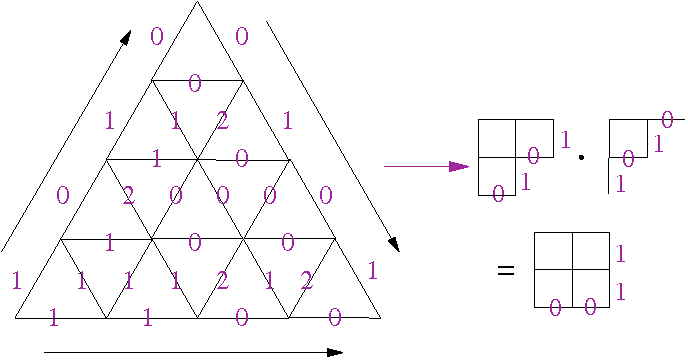
\includegraphics[scale=.7]{PuzzleFilled}\end{center}

In general, there may be either none or several.  Each valid puzzle contributes a term to the product in $H^*(Gr(k,n))$.

\end{frame} 



%-------------------------------------------%



\begin{frame}{The Rim Hook Rule}

\textbf{The Idea:} Compute $QH^*(Gr(k,n))$ from $H^*(Gr(k,\textcolor{blue}{2n-k}))$, where all products of $k \times (n-k)$ boxes ``fit'', and then remove rim hooks in exchange for the quantum parameter.

%\pause

\vskip 10pt

\begin{example}
To compute $\sigma_{\tableau[Yp]{\\}} \star \sigma_{\tableau[Yp]{& \\ & \\}}$ in $QH^*(Gr(2,4))$, first compute the classical product in $H^*(Gr(2,\textcolor{blue}{6}))$:

\[ \tableau[Ys]{\\} \cdot \tableau[Ys]{& \\ & \\} = \tableau[Ys]{&&\\ & \\}\ %\pause 
\mapsto \  \tableau[Ys]{& \textcolor{red}{\times} &  \textcolor{red}{\times} \\  \textcolor{red}{\times} &  \textcolor{red}{\times} \\} = q\ \tableau[Ys]{\\} \]

Then remove all possible $4$-rim hooks, picking up a (signed) power of $q$ for each rim hook removed. % \pause 
This gives
\[ \sigma_{\tableau[Yp]{\\}} \star \sigma_{\tableau[Yp]{& \\ & \\}} = q\sigma_{\tableau[Yp]{\\}}
\]

\end{example}

\end{frame}




%-------------------------------------------%

\begin{frame}{Equivariant Rim Hook Rule}


\begin{theorem}[Bertiger, M--, Taipale] The following algorithm gives quantum equivariant products in $QH^*_T(Gr(k,n))$: %\pause
\begin{itemize} 
\item Take classical product of factorial Schur functions (do equivariant Littlewood-Richardson in ``large enough'' Grassmannian) %\pause
\item In the quantum ideal, $\sigma_{\lambda} = (-1)^{\epsilon} q^d \sigma_{\nu}$ if we can remove $d$ $n$-rimhooks from $\lambda$ to get $\nu$ and the $n$-core $c(\nu)$ fits in $k \times (n-k)$ rectangle. %\pause
\item \textcolor{red}{Reduce equivariant coefficents by $t_i \mapsto t_{i \mod n}$} %\pause
\item Result gives quantum equivariant product of Schubert classes.
\end{itemize}\end{theorem}


\end{frame}


%-------------------------------------------%

\begin{frame}{Cyclic Factorial Schur Polynomials}

Symmetric function versions of the Peterson isomorphism:
\medskip
\medskip

\begin{tabular}{|c|c|}
\hline
$QH^*(G/B)$ & $H_*(Gr_G)$ \\ 
\hline
Schubert polynomials & $k$-Schur polynomials \\
\hline
\multicolumn{2}{|c|}{} \\
\hline
$QH_T^*(G/B)$ & $H^T_*(Gr_G)$ \\ 
\hline 
double Schubert polynomials & double $k$-Schur polynomials\\
\hline
\multicolumn{2}{|c|}{} \\
\hline
$QH_T^*(Gr(k,n))$ & $H^T_*(Gr_G)/J$ \\ 
\hline 
cyclic factorial Schurs & ???\\
\hline
\end{tabular}


\end{frame} 


%-------------------------------------------%





\end{document}
